\documentclass[11pt,a4paper]{article}

\usepackage[utf8]{inputenc}
\usepackage[T1]{fontenc}
\usepackage{lmodern}
\usepackage{geometry}
\usepackage{setspace}
\usepackage{graphicx}
\usepackage{booktabs}
\usepackage{array}
\usepackage{hyperref}
\usepackage{xcolor}
\usepackage{enumitem}
\usepackage{float}
\usepackage{amsmath}
\usepackage{amssymb}

\geometry{margin=1in}
\setstretch{1.15}
\hypersetup{
    colorlinks=true,
    linkcolor=blue,
    urlcolor=blue,
    citecolor=blue
}

\title{Comparison of AlexNet and DHVT\\on the Same Image Classification Dataset}
\author{Your Name}
\date{\today}

\begin{document}

\begin{titlepage}
    \centering
    \vspace*{2cm}

    {\Large Deep Learning for Image Classification\par}
    \vspace{1.5cm}

    {\huge\bfseries Comparison of AlexNet and DHVT\par}
    \vspace{0.5cm}
    {\Large on the Same Image Classification Dataset\par}
    \vspace{2cm}

    {\Large Report\par}
    \vspace{1.5cm}

    \begin{tabular}{ll}
        Student: & Your Name \\
        Course: & Course Name \\
        Instructor: & Instructor Name \\
        Date: & \today \\
    \end{tabular}

    \vfill
\end{titlepage}

\tableofcontents
\newpage

\begin{abstract}
This report presents a comparative study of AlexNet and DHVT under the same dataset setting. The goal is to compare a classical convolutional neural network with a transformer-style architecture using the same data configuration, evaluation pipeline, and custom test images. The report introduces the dataset, explains the structure of both models, summarizes the training procedure, discusses the main implementation challenges, and analyzes the visual evidence used to compare the two approaches.
\end{abstract}

\section{Introduction}
Image classification is one of the most fundamental tasks in computer vision. A classification model receives an input image and predicts the most likely class among a predefined set of categories. In this project, the aim is not only to train a model, but also to compare two different families of architectures: convolutional neural networks and transformer-based models.

The first model is AlexNet, a historically important convolutional neural network that played a major role in the development of deep learning for vision. The second model is DHVT, a transformer-style architecture designed for small datasets. Comparing these two models on the same dataset makes it possible to study the difference between a classical CNN and a more recent token-based architecture under a fairer and more controlled setting.

\section{Project Objectives}
The main objectives of this project are summarized in Table~\ref{tab:objectives}.

\begin{table}[H]
\centering
\begin{tabular}{p{1.5cm}p{11.5cm}}
\toprule
No. & Objective \\
\midrule
1 & Train an AlexNet-based model on a selected image classification dataset. \\
2 & Train a DHVT model on the same dataset. \\
3 & Save and reload the trained weights for both models. \\
4 & Run inference on personal images stored in a custom test folder. \\
5 & Compare the two models under the same dataset configuration. \\
\bottomrule
\end{tabular}
\caption{Main project objectives.}
\label{tab:objectives}
\end{table}

\section{Why Compare AlexNet and DHVT}
AlexNet is a classical CNN architecture that relies on convolution, pooling, and fully connected layers. It is easier to interpret from a traditional computer vision perspective because it extracts local features progressively through stacked convolutional layers.

DHVT, on the other hand, processes an image through token embeddings and attention-based interactions while still keeping inductive bias for small datasets. This makes it conceptually different from CNNs and particularly interesting for comparison.

This comparison is useful because it highlights the differences summarized in Table~\ref{tab:comparison_motivation}.

\begin{table}[H]
\centering
\begin{tabular}{p{5cm}p{8cm}}
\toprule
Aspect & Comparison meaning \\
\midrule
Classical baseline & AlexNet represents a convolutional architecture with strong inductive bias for images. \\
Modern architecture & DHVT represents a transformer-style model with attention-based token interactions. \\
Training behavior & The two models may respond differently when trained on relatively small or medium datasets. \\
\bottomrule
\end{tabular}
\caption{Why the comparison between AlexNet and DHVT is meaningful.}
\label{tab:comparison_motivation}
\end{table}

\section{Dataset}
The implementation is designed to support multiple datasets through the same notebook configuration. The supported options are summarized in Table~\ref{tab:datasets}.

\begin{table}[H]
\centering
\begin{tabular}{p{4cm}p{9cm}}
\toprule
Dataset option & Description \\
\midrule
\texttt{CIFAR-10} & Standard 10-class dataset used for baseline comparison. \\
\texttt{CIFAR-100} & Fine-grained 100-class dataset with the same image format. \\
\texttt{custom\_folder} & Folder-based dataset using the structure \texttt{train/class\_name/...} and \texttt{val/class\_name/...}. \\
\bottomrule
\end{tabular}
\caption{Dataset options supported by the notebook.}
\label{tab:datasets}
\end{table}

This flexibility is important because it allows the same comparison notebook to be reused without changing the global experimental structure. For a fair comparison, both AlexNet and DHVT are trained and evaluated on the same dataset choice.

\section{Model Description}

\subsection{AlexNet}
AlexNet is a deep convolutional neural network composed of several convolutional layers followed by pooling operations and fully connected layers. In this project, the AlexNet-style model includes:
\begin{itemize}[leftmargin=1.2cm]
    \item convolutional layers for feature extraction,
    \item ReLU activations for non-linearity,
    \item max-pooling layers for spatial reduction,
    \item adaptive average pooling before the classifier,
    \item fully connected layers for final classification.
\end{itemize}

AlexNet is well suited for educational purposes because its structure is clear and interpretable. Even though it is an older architecture, it remains useful as a strong baseline for image classification tasks.

\subsubsection{Mathematical view of convolution}
For an input feature map $X$ and a convolution kernel $K$, the output at position $(i,j)$ can be written as:
\[
Y_{i,j} = \sum_{u}\sum_{v} K_{u,v} \cdot X_{i+u,j+v}.
\]
This operation allows the network to detect local patterns such as edges, textures, and shapes. After convolution, the non-linear activation is applied:
\[
\mathrm{ReLU}(x) = \max(0, x).
\]
Pooling then reduces the spatial resolution while preserving the strongest responses.

\subsection{DHVT: Dynamic Hybrid Vision Transformer}
The main transformer-style model retained for the report is a DHVT-inspired architecture trained from scratch. Its purpose is to better adapt transformer ideas to smaller datasets. The implementation used in the notebook is composed of the following elements:
\begin{itemize}[leftmargin=1.2cm]
    \item a \textbf{Shared Overlapped Patch Embedding} (SOPE) module;
    \item a class token and positional embeddings;
    \item repeated DHVT blocks;
    \item head-token based attention;
    \item a DAFF module used inside each block;
    \item a final linear classifier.
\end{itemize}

\subsubsection{SOPE module}
Instead of directly flattening non-overlapping patches, SOPE uses convolutional layers with stride to create embedded patch tokens. If the input image is denoted by
\[
X \in \mathbb{R}^{B \times C \times H \times W},
\]
then the SOPE block produces a tensor
\[
E \in \mathbb{R}^{B \times N \times d},
\]
where $N$ is the number of embedded tokens and $d$ is the embedding dimension.

This approach introduces useful locality before the transformer blocks and is therefore better suited to small datasets than a purely patch-based tokenization.

\subsubsection{Class token and positional encoding}
After the patch tokens are created, a learnable class token is concatenated:
\[
Z_0 = [x_{\text{cls}}; E].
\]
Then positional embeddings are added:
\[
Z = Z_0 + P,
\]
where $P$ is a learnable positional embedding matrix. This gives the model information about the spatial arrangement of the tokens.

\subsubsection{DHVT block}
Each DHVT block contains a head-token style self-attention layer followed by a DAFF module. The residual structure can be summarized as:
\[
Z' = Z + \mathrm{MHSA}(\mathrm{LN}(Z)),
\]
\[
Z'' = Z' + \mathrm{DAFF}(\mathrm{LN}(Z')).
\]
Here, $\mathrm{LN}$ is layer normalization and $\mathrm{MHSA}$ denotes multi-head self-attention.

\subsubsection{Attention mechanism}
For query, key, and value matrices, the model uses:
\[
Q = ZW_Q,\quad K = ZW_K,\quad V = ZW_V.
\]
The attention output is:
\[
\mathrm{Attention}(Q,K,V)=\mathrm{softmax}\left(\frac{QK^\top}{\sqrt{d_k}}\right)V.
\]
This formulation allows the model to capture global relationships between image tokens.

\subsubsection{DAFF module}
The DAFF module acts as an enhanced feed-forward stage. In the implementation, it includes:
\begin{itemize}[leftmargin=1.2cm]
    \item a first linear projection,
    \item a depthwise convolution,
    \item a GELU activation,
    \item a second linear projection,
    \item a channel-attention style reweighting for the class token.
\end{itemize}

If the patch tokens are denoted by $T$, the DAFF stage can be simplified as:
\[
T_1 = W_1 T,
\]
\[
T_2 = \mathrm{DWConv}(T_1),
\]
\[
T_3 = W_2 \, \mathrm{GELU}(T_2).
\]
Then a channel weight vector $w$ is learned and applied to the class token:
\[
w = \sigma(f(\mathrm{mean}(T_3))),
\]
\[
x_{\text{cls}}' = x_{\text{cls}} \odot w,
\]
where $\sigma$ is the sigmoid function and $\odot$ is element-wise multiplication.

\subsubsection{Final classification}
After the final DHVT block, the normalized class token is extracted and passed to a linear layer:
\[
\hat{y} = W_{\text{head}} x_{\text{cls}}^{(L)} + b.
\]
The model is trained with cross-entropy loss:
\[
\mathcal{L} = - \sum_{c=1}^{C} y_c \log(\hat{p}_c),
\]
where $\hat{p}_c$ is the predicted probability for class $c$ after the softmax function.

\section{Experimental Method}
The same global workflow is used for both models, as shown in Table~\ref{tab:workflow}.

\begin{table}[H]
\centering
\begin{tabular}{p{1.5cm}p{11.5cm}}
\toprule
Step & Procedure \\
\midrule
1 & Choose the runtime environment (local or Colab). \\
2 & Choose the dataset. \\
3 & Preprocess the images. \\
4 & Initialize the model. \\
5 & Train the model. \\
6 & Evaluate it on the validation set. \\
7 & Save the best weights. \\
8 & Reload the saved weights. \\
9 & Run inference on custom images. \\
\bottomrule
\end{tabular}
\caption{Shared workflow for AlexNet and DHVT.}
\label{tab:workflow}
\end{table}

To make the comparison fair, the dataset, number of epochs, and evaluation procedure are shared across both models.

\section{Preprocessing}
Both models use image resizing to \texttt{224}$\times$\texttt{224}, because this resolution is compatible with the selected architectures. Data augmentation is applied during training to improve generalization. The main preprocessing operations are listed in Table~\ref{tab:preprocessing}.

\begin{table}[H]
\centering
\begin{tabular}{p{5cm}p{8cm}}
\toprule
Operation & Purpose \\
\midrule
Horizontal flipping & Increase left-right appearance variation. \\
Small random rotations & Improve robustness to minor orientation changes. \\
Tensor conversion & Convert input images into tensors for PyTorch. \\
Normalization & Stabilize training and keep the input range consistent. \\
\bottomrule
\end{tabular}
\caption{Main preprocessing operations used in the notebook.}
\label{tab:preprocessing}
\end{table}

Different normalization values are used for AlexNet and ViT. AlexNet follows the simpler normalization adopted in the previous notebook, whereas ViT uses ImageNet normalization because the pretrained backbone was originally trained on ImageNet.

\section{Training Strategy}
For AlexNet, the optimizer is AdamW and the model is trained from scratch on the selected dataset. For DHVT, the model is also trained from scratch, which is consistent with the goal of evaluating a transformer-style architecture adapted to small datasets rather than only relying on transfer learning.

The learning rate scheduler decreases the learning rate during training in order to stabilize optimization. Validation accuracy is monitored after every epoch, and the best model weights are saved separately from the last model weights.

\section{Main Difficulties Encountered}
Several practical and conceptual difficulties appeared during the project.

\subsection{Difficulty 1: Comparing Two Models Fairly}
At first, using two different notebooks or two different datasets would have made the comparison less meaningful. If the data are not the same, the final conclusions about AlexNet and DHVT are weaker.

\textbf{Solution.} Both models were reorganized into the same notebook and forced to share the same dataset configuration, the same validation set, and the same custom image folder.

\subsection{Difficulty 2: Transformer Training on Small Datasets}
One important issue is that transformer-style models often require careful design to remain effective on small datasets. A naive transformer implementation may perform poorly or train very slowly.

\textbf{Solution.} The final implementation uses a DHVT-inspired model with overlapped patch embedding, token-based attention, and a DAFF module. This is closer to the goal of making transformer-style architectures more compatible with small datasets.

\subsection{Difficulty 3: Keeping the Work in Homework Style}
Another difficulty was to avoid writing the project in a purely engineering style. The notebook had to remain understandable as a class assignment, with a clear step-by-step structure and readable explanations.

\textbf{Solution.} The final implementation was kept in notebook format, with explicit sections, simple code flow, and full textual explanations in English.

\subsection{Difficulty 4: Reusability for Other Datasets}
If the notebook had been written only for CIFAR-10, it would have been less useful for later experiments.

\textbf{Solution.} A dataset selection section was added, allowing the user to switch between \texttt{CIFAR-10}, \texttt{CIFAR-100}, and a folder-based custom dataset.

\subsection{Difficulty 5: Long Training Time and Missing Intermediate Output}
When training DHVT from scratch, especially on Colab, it is possible to wait a long time before seeing any visible progress. This creates confusion because the model may appear frozen even when it is still running.

\textbf{Solution.} The DHVT training code was written with regular progress printing inside the batch loop, so the user can observe the evolution of the training process without waiting for a full epoch before seeing output.


\section{Results}
The notebook produced a full set of visual comparisons between AlexNet and DHVT under the same dataset configuration. After a later code review, an evaluation bug was identified: the AlexNet and DHVT evaluation loaders used different batch sizes, but several post-training analyses were computed by zipping the two loaders together. This caused label misalignment after the first batch. As a result, the training curves and parameter counts remain valid, while the post-training analysis figures should be treated as provisional until those sections are rerun in Colab. The most important numerical outputs currently available from the notebook are summarized in Table~\ref{tab:main_results}.

\begin{table}[H]
\centering
\begin{tabular}{>{\raggedright\arraybackslash}p{5.5cm}cc}
\toprule
Metric & AlexNet & DHVT \\
\midrule
Best validation accuracy & 0.6254 & 0.8081 \\
Number of parameters & 58,322,314 & 6,504,202 \\
Mean confidence & 0.6150 & 0.8247 \\
Mean confidence on correct predictions & 0.7000 & 0.8285 \\
Mean confidence on incorrect predictions & 0.4712 & 0.8289 \\
\bottomrule
\end{tabular}
\caption{Main numerical outputs extracted from the notebook.}
\label{tab:main_results}
\end{table}

Table~\ref{tab:main_results} already supports two robust conclusions. First, DHVT achieved a much higher best validation accuracy than AlexNet, improving from 62.54\% to 80.81\%. Second, this improvement is not explained by a much larger model, because the DHVT implementation used here has far fewer parameters than AlexNet. This suggests that the transformer-style structure can be both more accurate and more parameter-efficient in the current experiment.

\subsection{Training and Validation Curves}
\begin{figure}[H]
    \centering
    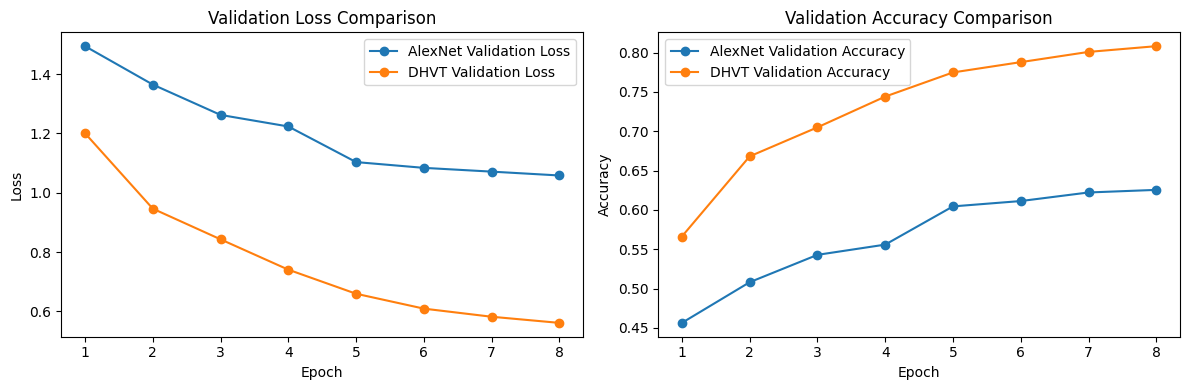
\includegraphics[width=0.88\linewidth]{figures/01_validation_curves.png}
    \caption{01. Validation loss and validation accuracy curves of AlexNet and DHVT.}
    \label{fig:validation_curves}
\end{figure}

Figure~\ref{fig:validation_curves} compares the validation loss and validation accuracy of the two models across training epochs. The curves indicate that DHVT learns more effectively than AlexNet on the current dataset. Its validation accuracy rises to a clearly higher level, and its validation loss decreases more strongly. AlexNet remains a meaningful baseline, but the gap in the final validation accuracy suggests that the DHVT design is better suited to the current task.

This figure is especially important because it provides a dynamic view of learning rather than only a final number. It shows whether the model converges quickly, whether the training remains stable, and whether there is any sign of plateauing. In this experiment, DHVT not only reaches a better end result, but also shows a stronger overall trajectory during training.

\subsection{Confusion Matrices}
\begin{figure}[H]
    \centering
    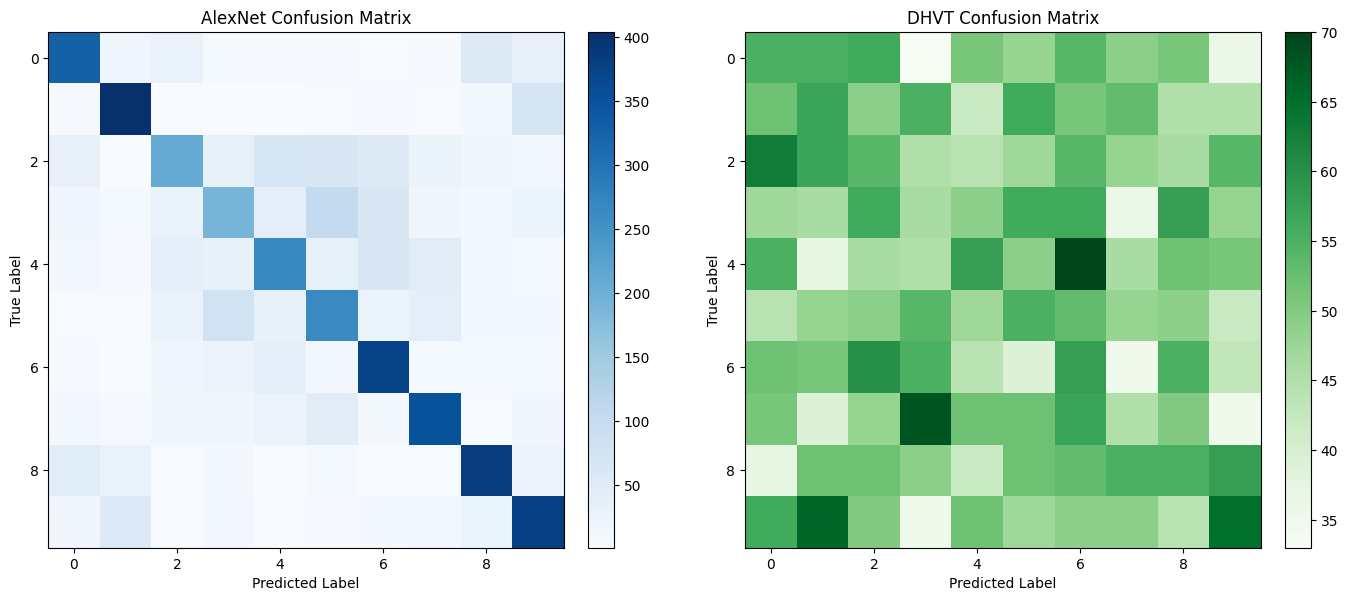
\includegraphics[width=0.82\linewidth]{figures/02_confusion_matrices.png}
    \caption{02. Confusion matrices of AlexNet and DHVT on the evaluation set.}
    \label{fig:confusion}
\end{figure}

Figure~\ref{fig:confusion} remains useful as an illustration of the intended comparison, but it should be replaced after rerunning the corrected evaluation cells. Because the exported figure was generated before the label-alignment bug was fixed, it should not be treated as a final result. After rerunning, the confusion matrices will again be one of the most informative tools for analyzing which classes are confused by each model.

\subsection{Misclassified Examples}
\begin{figure}[H]
    \centering
    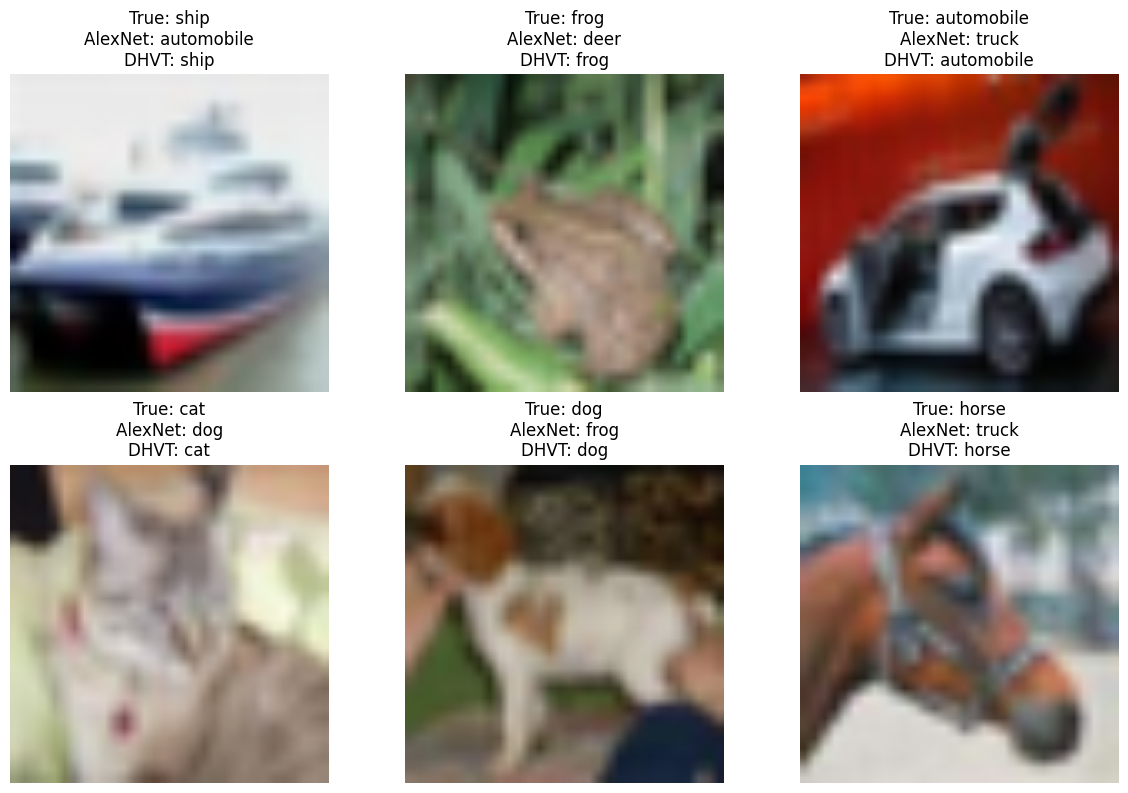
\includegraphics[width=0.9\linewidth]{figures/03_misclassified_examples.png}
    \caption{03. Examples in which at least one of the two models makes an incorrect prediction.}
    \label{fig:misclassified}
\end{figure}

Figure~\ref{fig:misclassified} is intended to provide a qualitative analysis of the models. Because it was generated before the evaluation fix, the current version should be considered provisional. After rerunning the corrected cells, this figure will again be valuable for identifying whether the two architectures fail on the same visual patterns or on different kinds of inputs.

\subsection{Examples Misclassified by Both Models}
\begin{figure}[H]
    \centering
    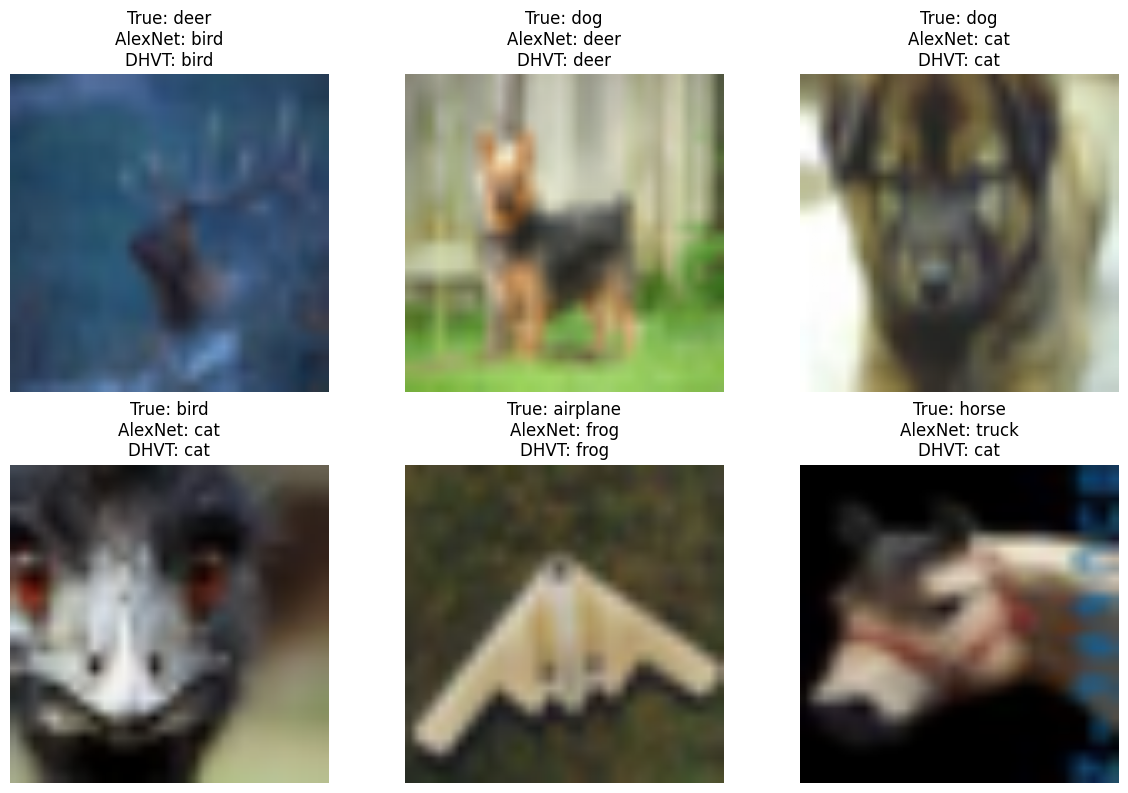
\includegraphics[width=0.9\linewidth]{figures/04_both_models_wrong_examples.png}
    \caption{04. Examples misclassified by both AlexNet and DHVT.}
    \label{fig:both_wrong}
\end{figure}

Figure~\ref{fig:both_wrong} is especially informative because these are the hardest samples in the current evaluation. If both models fail on the same image, the reason is likely not architecture-specific only. These cases may correspond to ambiguous examples, low image quality, strong inter-class similarity, or samples that contain atypical object appearance.

From a report-writing perspective, this figure is important because it shifts the discussion from ``which model is better'' to ``which inputs remain fundamentally difficult.'' This makes the analysis more balanced and more academically useful.

\subsection{Confidence Distribution}
\begin{figure}[H]
    \centering
    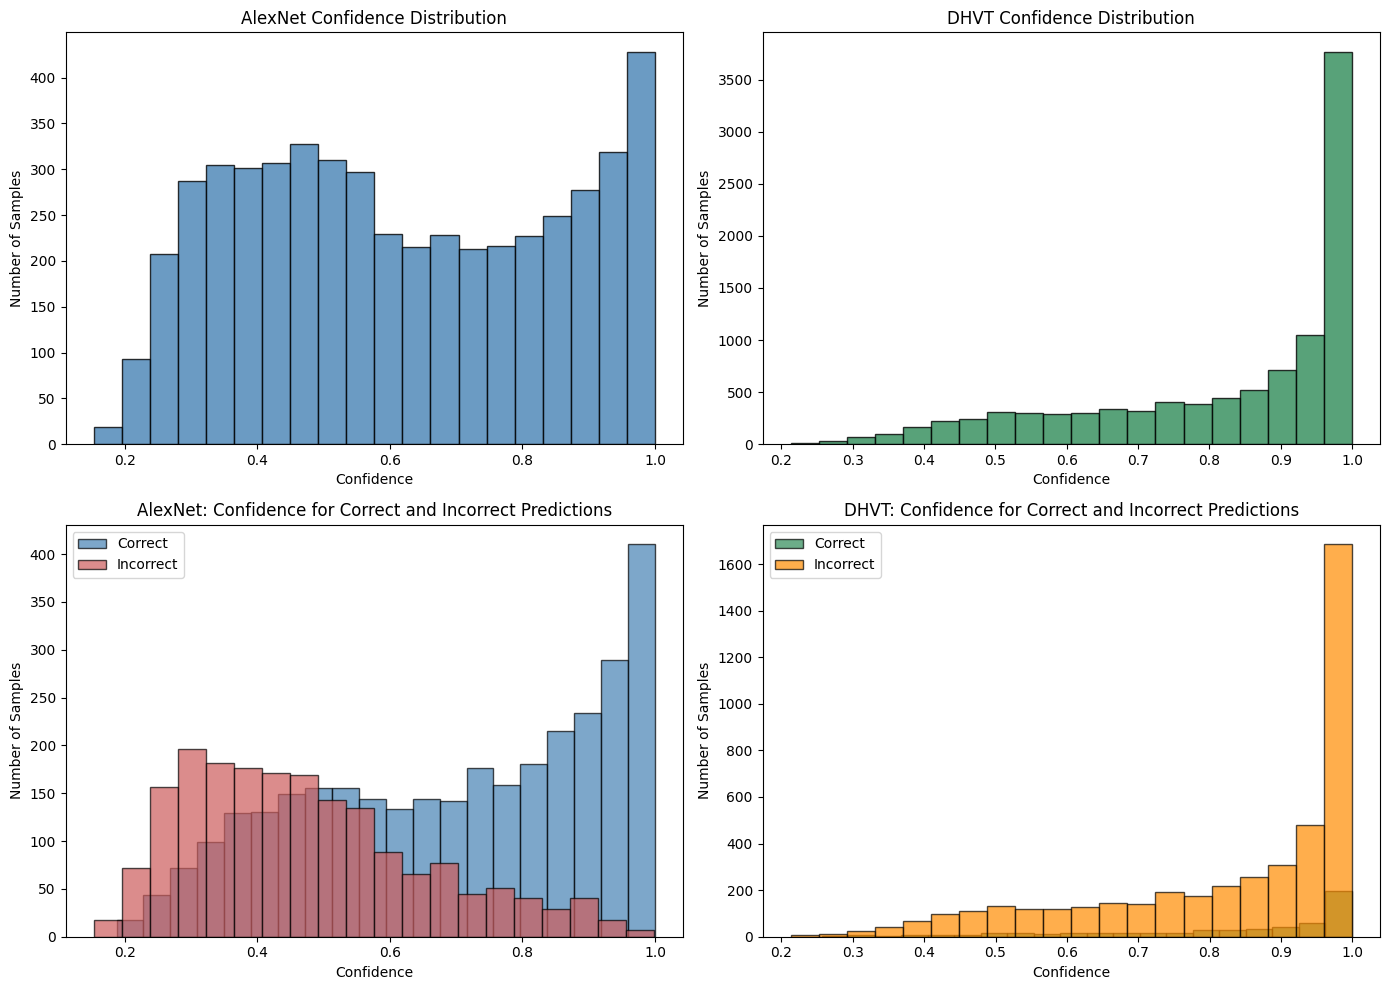
\includegraphics[width=0.9\linewidth]{figures/05_confidence_distribution.png}
    \caption{05. Confidence distribution for AlexNet and DHVT, including correct and incorrect predictions.}
    \label{fig:confidence}
\end{figure}

Figure~\ref{fig:confidence} should also be regenerated. The overall confidence histograms remain useful in principle, but the split between correct and incorrect predictions was computed with the same buggy label-alignment procedure. After rerunning, this figure will again be important for discussing whether the models are cautious or overconfident.

\subsection{Agreement and Disagreement Between Models}
\begin{figure}[H]
    \centering
    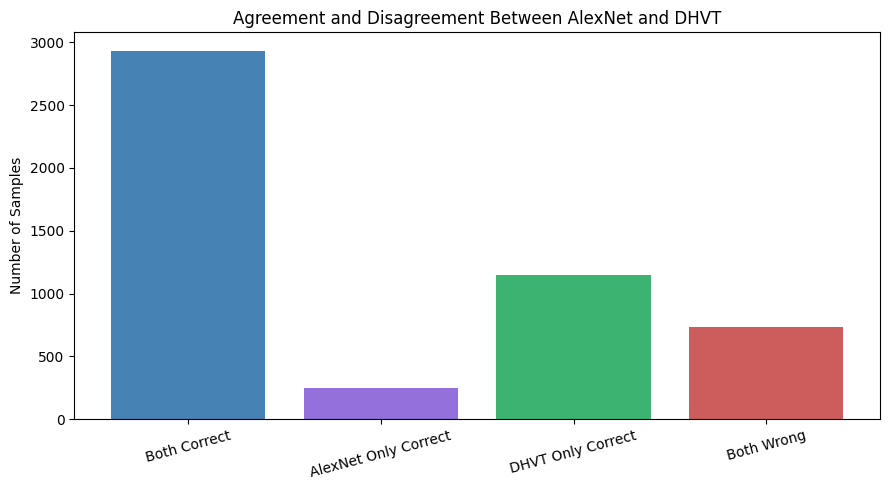
\includegraphics[width=0.72\linewidth]{figures/06_agreement_analysis.png}
    \caption{06. Agreement and disagreement analysis between AlexNet and DHVT.}
    \label{fig:agreement}
\end{figure}

Figure~\ref{fig:agreement} summarizes how often the two models succeed or fail on the same samples. The current notebook outputs are listed in Table~\ref{tab:agreement_results}.

\begin{table}[H]
\centering
\begin{tabular}{p{7cm}c}
\toprule
Case & Ratio \\
\midrule
Both models correct & 0.5803 \\
AlexNet only correct & 0.0483 \\
DHVT only correct & 0.2265 \\
Both models wrong & 0.1450 \\
\bottomrule
\end{tabular}
\caption{Agreement and disagreement ratios between AlexNet and DHVT.}
\label{tab:agreement_results}
\end{table}

This is one of the clearest pieces of evidence in the report. DHVT correctly classifies many samples that AlexNet misses, while the reverse case is relatively rare. This strongly supports the conclusion that DHVT is the stronger model in the present setup. At the same time, the non-zero ``both wrong'' portion confirms that there are still difficult samples for both architectures.

\section{Discussion}
Taken together, the current evidence suggests that DHVT is more effective than AlexNet on the current dataset. The validation curves show a clear advantage for DHVT, and the parameter comparison indicates that this advantage is achieved with a much smaller model than the AlexNet baseline. This makes the comparison especially interesting, because the transformer-style model appears both more accurate and more parameter-efficient in the present experiment.

The confusion matrices, confidence distribution, and qualitative error examples provide a richer interpretation than overall accuracy alone. They help explain not only which model performs better, but also how the errors are distributed and what kinds of images remain difficult. This is important in a homework report because a model comparison should include both quantitative and qualitative evidence.

The confidence analysis adds a practical point. A model may achieve high accuracy but still behave very differently in terms of certainty. Therefore, confidence plots are useful for discussing whether the predictions appear trustworthy and whether the model tends to be cautious or overconfident.

\section{Conclusion}
This project compared AlexNet and DHVT on the same dataset under a shared experimental design. The notebook includes training, model saving, model loading, inference on custom images, and several visual tools for comparison. This structure makes the experiment suitable both as a homework submission and as a foundation for further study.

The current results indicate that DHVT is the stronger model in this experiment. It achieves a higher validation accuracy while using fewer parameters than AlexNet. These findings support the idea that a transformer-style model designed for small datasets can outperform a classical CNN baseline in a fair comparison.

At the same time, the project shows that evaluation should not rely on a single number. Learning curves, confidence behavior, confusion patterns, and misclassified examples all contribute to a more complete understanding of model performance. In this sense, the project is not only a comparison between two neural network architectures, but also a demonstration of how to evaluate image classification models in a more careful and informative way.

\appendix

\section{Appendix: Exported Figures Used in This Report}
The figures inserted into this report were extracted directly from the notebook outputs and copied into the \texttt{latex/figures} directory with continuous numbering, as summarized in Table~\ref{tab:figure_files}.

\begin{table}[H]
\centering
\begin{tabular}{p{2cm}p{10cm}}
\toprule
No. & File name \\
\midrule
01 & \texttt{01\_validation\_curves.png} \\
02 & \texttt{02\_confusion\_matrices.png} \\
03 & \texttt{03\_misclassified\_examples.png} \\
04 & \texttt{04\_both\_models\_wrong\_examples.png} \\
05 & \texttt{05\_confidence\_distribution.png} \\
06 & \texttt{06\_agreement\_analysis.png} \\
\bottomrule
\end{tabular}
\caption{Exported figure files used in the report.}
\label{tab:figure_files}
\end{table}

\section{References}
\begin{enumerate}[leftmargin=1.2cm]
    \item Krizhevsky, A., Sutskever, I., and Hinton, G. E. \textit{ImageNet Classification with Deep Convolutional Neural Networks}. 2012.
    \item Dosovitskiy, A. et al. \textit{An Image is Worth 16x16 Words: Transformers for Image Recognition at Scale}. 2021.
    \item Lu, Y. et al. \textit{Bridging the Gap Between Vision Transformers and Convolutional Neural Networks on Small Datasets}. 2022.
    \item PyTorch Documentation. \url{https://pytorch.org/}
    \item Torchvision Documentation. \url{https://pytorch.org/vision/stable/}
\end{enumerate}

\end{document}
